% Author : Alain Matthes
% Encoding : UTF8
% Engine : PDFLaTeX
\documentclass[]{article}
\usepackage[utf8]{inputenc} 
\usepackage[usenames,dvipsnames]{xcolor}
\usepackage{fullpage}
\usepackage[upright]{fourier}
\usepackage{tkz-berge}
\thispagestyle{empty}

\begin{document}
	
\tikzstyle{EdgeStyle}= [thick,%
                        double          = orange,%
                        double distance = 1pt] 
\begin{center}

    \tikzstyle{VertexStyle}=[shape        = circle,
                             shading      = ball,
                             ball color   = green!30,
                             minimum size = 24pt,
                             draw]
    \SetVertexLabel
    \tikzstyle{EdgeStyle}= [color=red!30,
                            double= green!50!black,
                            double distance = 2pt] 
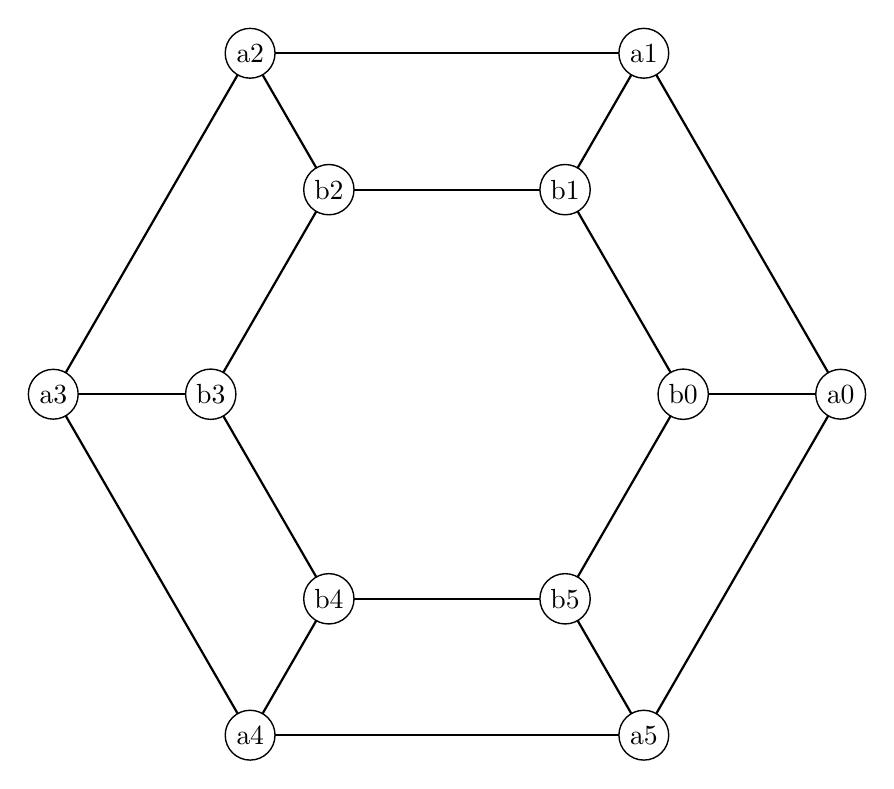
\begin{tikzpicture}
\grPrism[RA=5,RB=3]{6}%
\end{tikzpicture}

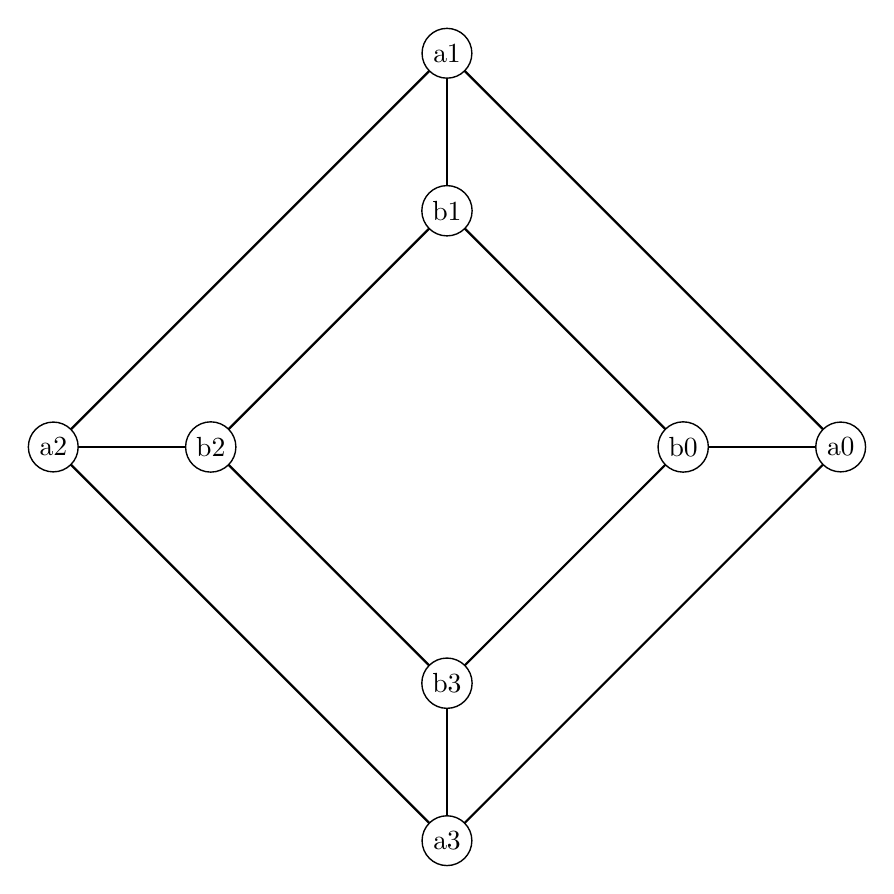
\begin{tikzpicture}
\grPrism[RA=5,RB=3]{4}%
\end{tikzpicture}


\end{center}

\end{document}